% !TEX root = morphkasten.tex

\section{Beladen}


%##############
\subsection{Arm ohne Knick}

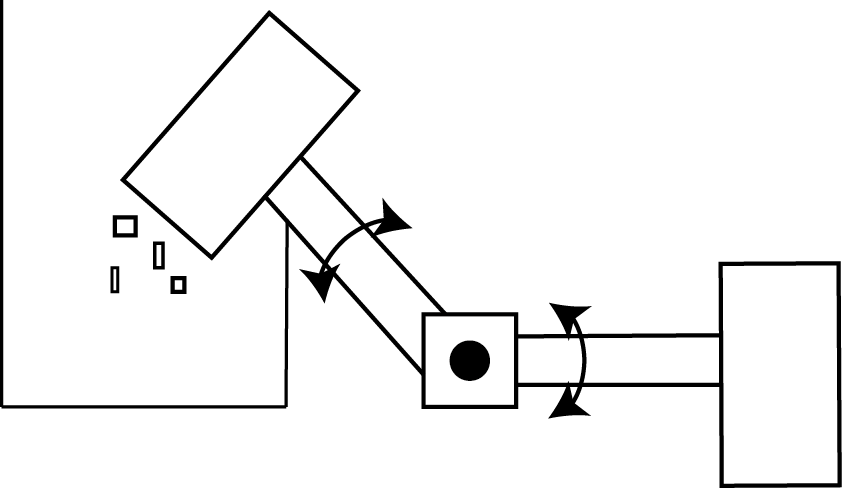
\includegraphics[width=0.5\textwidth]{fig/Beladen_1.png}

\begin{table}[h]
\begin{tabular}{p{0.5\textwidth} | p{0.5\textwidth}}


 \textbf{Vorteile} & \textbf{Nachteile} \\ \hline
	 
\begin{itemize}
\item nur ein Motor nötig für die gesamte Funktion
\item simple Lösung
\item komplette Entladung ohne Probleme möglich
\end{itemize}

 
 &
 
\begin{itemize}
\item keine
\end{itemize}

\end{tabular}
\end{table}

\begin{table}[h]
\begin{tabular}{p{0.5\textwidth}p{0.5\textwidth}}


 \textbf{Risiken} & \\ \hline
	 
\begin{itemize}
\item Länge von Drehgelenk zu Greifer Ende muss optimal gewählt werden
\item zu hohe Motorbelastung
\end{itemize}
 
\end{tabular}
\end{table}

\pagebreak


%##############
\subsection{Knickarm}

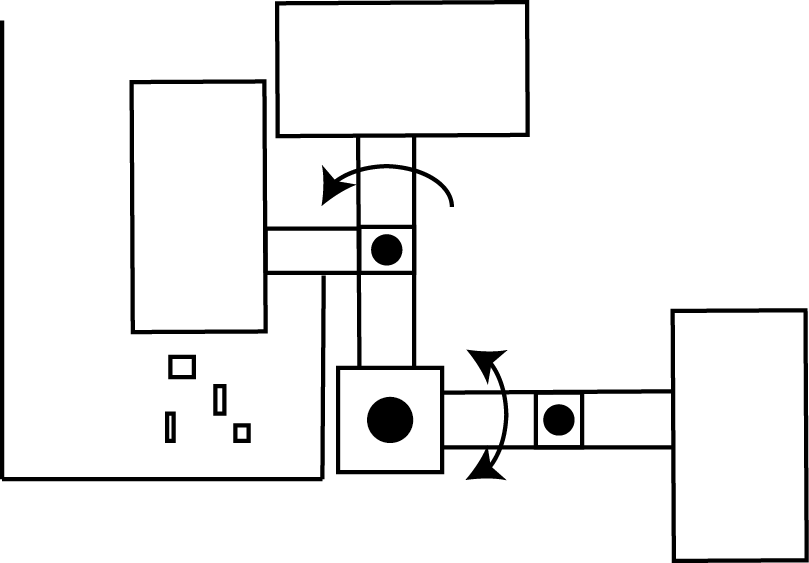
\includegraphics[width=0.5\textwidth]{fig/Beladen_2.png}

\begin{table}[h]
\begin{tabular}{p{0.5\textwidth} | p{0.5\textwidth}}


 \textbf{Vorteile} & \textbf{Nachteile} \\ \hline
	 
\begin{itemize}
\item Kompakte Bauweise (weniger breit als vorherige Variante)
\item Entladung einfach möglich 
\end{itemize}

 
 &
 
\begin{itemize}
\item 2 Motoren notwendig
\item aufwändiger Bewegungsablauf
\end{itemize}

\end{tabular}
\end{table}

\begin{table}[h]
\begin{tabular}{p{0.5\textwidth}p{0.5\textwidth}}


 \textbf{Risiken} & \\ \hline
	 
\begin{itemize}
\item zu frühes knicken (Schüttgut landet nicht in Behälter) 
\end{itemize}
 
\end{tabular}
\end{table}

\pagebreak